\documentclass[12pt,a4paper]{article}

\makeatletter
\def\input@path{{/home/maenwe/Master_CSM/modèle_cours_latex}}
\makeatother

\usepackage{prise_de_note}
\usepackage{subcaption}
\usepackage{graphicx}
\usepackage{tkz-euclide}
\usetikzlibrary{intersections}

\graphicspath{{/home/maenwe/Master_CSM/modèle_cours_latex}}

\begin{document}
	\pagenumbering{gobble}
	
	\begin{titlepage}
		\centering
		
		% Logo
		\begin{figure}[h]
			\centering
			% Ajustez la largeur si besoin (ex: 0.4 ou 0.6)
			
\includegraphics[width=0.5\textwidth]{logo.png} 
		\end{figure}
		
		\vspace{2cm}
		
		% Filet horizontal du haut
		\rule{\linewidth}{0.5mm} \\[0.4cm]
		
		% Titre
		{\color{bleuTitre} \Huge \bfseries Consistance de gradients discrets sur des maillages non-structurés 2D} \\[0.4cm]
		
		% Filet horizontal du bas
		\rule{\linewidth}{0.5mm}
		
		\vspace{1.5cm}
		
		{\Large Rapport de stage}
		
		\vfill
		
		% Bloc Informations
		\begin{minipage}{0.45\textwidth}
			\begin{flushleft} \large
				\textbf{Encadrant :} \\
				Ludovic \textsc{MARTAUD}
			\end{flushleft}
		\end{minipage}
		\hfill
		\begin{minipage}{0.45\textwidth}
			\begin{flushright} \large
				\textbf{Étudiant :} \\
				Nathan \textsc{HASCOET}
			\end{flushright}
		\end{minipage}
		
		\vspace{2cm}
		
		% Date
		{\large \today}
		
	\end{titlepage}
	
	\tableofcontents
	
	\newpage
	
	\pagenumbering{arabic}
	\setcounter{page}{1}
	
	\section{Introduction}	
	
	\subsection{Contexte}
	
	Ce stage s'est déroulé au sein de l'Institut de Recherche Mathématique de Rennes (IRMAR), un
	laboratoire de recherche fondamentale et appliquée en mathématiques, rattaché à l'Université de Rennes et au CNRS. L'IRMAR couvre un large spectre de thématiques, allant de l'analyse et la géométrie à la modélisation numérique et aux statistiques. Le stage a bénéficié du soutien financier du Centre Henri Lebesgue, un centre de recherche mathématique interrégional qui vise à promouvoir l'excellence scientifique, à renforcer la collaboration entre chercheurs et à soutenir la formation par la recherche dans le domaine des mathématiques.
	\par Dans le cadre des méthodes aux volumes finis, il est très intéressant de considérer le gradient de la solution discrète au pas $n$ pour pouvoir calculer la solution discrète au pas $n+1$ tel qu'il est fait dans la méthode d'Euler.
	\par Le sujet de ce stage porte sur l'étude de la consistance d'un gradient discret local défini dans l'article \cite{ludo} sur des maillages anisotrope non structuré en deux dimensions. Un maillage est dit anisotrope lorsqu'il présente des cellules allongées ou déformées dans certaines directions, contrairement à un maillage isotrope où les cellules sont régulières et uniformes. 
	\par Bien que les maillages anisotropes soient plus complexes à manipuler, de nombreux domaines à mailler, tels que des ailes d'avions par exemple, impose d'utiliser des maillages anisotropes pour pouvoir espérer les mailler, c'est pour cela que l'étude est faite sur un carré maillé par un maillage anisotrope.
	\par La structure du maillage (les angles formés et les longueurs des segments) et la façon dont est mesuré de ce maillage, impacte directement l'erreur de consistance de gradients discrets.	
	\par Une question émerge naturellement de ces considérations : 
	\begin{center}
		Ce gradient discret converge t'il et à quel ordre ?
	\end{center}
	
	\subsection{Modélisation du problème}
	
	\begin{center}
		\begin{tikzpicture}[line cap=round,line join=round,x=1.0cm,y=1.0cm, scale = 0.6]
			\clip(1.38,2.770816326530614) rectangle (15.776381418092914,12.74);
			\draw [line width=1.pt] (8.58,10.26)-- (8.8,4.78);
			\draw [line width=1.pt] (8.8,4.78)-- (3.72,4.74);
			\draw [line width=1.pt] (8.8,4.78)-- (12.42,3.02);
			\draw [line width=1.pt] (5.,12.)-- (8.58,10.26);
			\draw [line width=1.pt] (8.58,10.26)-- (13.74,11.74);
			\draw [line width=1.pt,dash pattern=on 1.5pt off 1.5pt] (6.08,8.84)-- (11.78,7.84);
			\draw (5.476625916870418,5.644081632653063) node[anchor=north west] {$C_i$};
			\draw (10.702151589242057,5.644081632653063) node[anchor=north west] {$C_j$};
			\draw [->,line width=0.8pt] (8.712203119196165,6.966940485477385) -- (9.631492956467849,7.003846281864205);
			\draw[color=black] (9.631492956467849,7.003846281864205) node[above] {$n_{ij}$};
			%% \draw[color=black] (8.840048899755503,7.15) node[above left] {$\Gamma_{ij}$};
			\draw [fill=black] (6.08,8.84) circle (2.0pt);
			%% \draw[decorate,decoration={brace}] (6.1632762836185835,10.05826530612245) -- (11.865965770171153,9.057857142857145);
			\draw[color=black] (6.1632762836185835,9.05826530612245) node {$x_i$};
			\draw [fill=black] (11.78,7.84) circle (2.0pt);
			\draw[color=black] (11.865965770171153,8.057857142857145) node {$x_j$};
			\draw [fill=black] (8.65514444157854,8.388220273407274) circle (2.0pt);
			\draw[color=black] (8.735305623471884,8.581326530612246) node[above right, yshift = -0.2cm] {$x_{ij}$};
			%node[above,xshift=-0.5cm, yshift=-0.2cm] {$x_{ij}$};
			\draw [fill=black] (8.69,7.52) circle (2.0pt);
			\draw[color=black] (8.770220048899757,7.70887755102041) node[above,xshift=-0.5cm, yshift=-0.5cm] {$\overline{x}_{ij}$};
			%% \draw [fill=xdxdff] (8.778392298328422,5.318228205273862) circle (2.5pt);
			\draw[color=black] (8.863325183374085,5.53357142857143) node[right] {$\Gamma_{ij}$};
		\end{tikzpicture}
		\captionof{figure}{Interface orientée $\Gamma_{ij}$ localisée entre deux cellules $C_i$ et $C_j$ d'un maillage non structuré $\mathcal{T}$ dans lequel $ \overline{x}_{ij}$ est le milieu de $\Gamma_{ij}$ avec $x_{ij} = \Gamma_{ij} \cap [x_i, x_j]$ où $x_i$ et $x_j$ sont les centres de gravités des cellules $C_i$ et $C_j$ respectivement.}
		\label{fig:EdgeWithGrandeurs}
	\end{center}
	
	Soit $\lambda_1$ la mesure de Lebesgue sur $\R$, et, $\lambda_2$ la mesure de Lebesgue sur $\R^2$ et $\left\{C_i; i\in [\![1,N]\!]  \right\} = \mathcal T$ un ensemble de polygone tel que les $C_i$ forment un pavage de $\R^2$. \par Puisque $\mathcal T$ permet de former un pavage du plan, pour tout $i \not= j$, $\Gamma_{i,j} = C_i \cap C_j$ (muni d'une orientation, de $C_i$ vers $C_j$) est soit vide, soit contient un unique point, soit est un segment. Ainsi pour tout $i \in \mathcal T$ et $j \in \mathcal N_i = \left\{j \in \mathcal T;\; \lambda_1\left(\Gamma_{i,j}\right)>0\right\}$, le vecteur $n$ est constant sur $\Gamma_{i,j}$ où $n(x)$ est unitaire, normal à $\Gamma_{i,j}$ en $x \in \Gamma_{i,j}$ et orienté de $C_i$ vers $C_j$. Dans la suite $n\Big|_{\Gamma_{i,j}}$ est noté $n_{i,j}$.\\
	
	Par abus de notation, $\lambda_1(\cdot)$ et $\lambda_2(\cdot)$ sont notés de la même manière : $|\cdot|$. Et par abus de notation, il est noté $i \in \mathcal T$ pour $C_i \in \mathcal T$.\\
	
	Dans la modélisation discrète de $u$ est pris constant sur chaque cellule $C_i$ et la valeur choisie est :
	\begin{equation}
		u_k = \dfrac1{\abs{C_k}}\displaystyle\int_{C_k} u(x)\dx,
	\end{equation}
	
	Pour la suite il est nécessaire d'introduire les deux quantités suivantes pour $i \in \mathcal T$, $j \in \mathcal{N}_i$ et $k \in \{i,j\}$ :	
	\begin{equation}
		d_{i,j} = d(x_i,x_j),
	\end{equation}
	\begin{equation}
		d_{k,ij} = d(x_k,x_{i,j}).
	\end{equation}
	\begin{equation}
		\lambda_{i,j} = \abs{\Gamma_{i,j}},
	\end{equation}
	
	et de la matrice de $\mathcal M_{2,2}(\R)$ suivante :
	et \begin{equation}
		M_i = I_2 - \dfrac1{\abs{C_i}}\displaystyle\sum_{j \in \mathcal N_i} \lambda_{i,j} {n_{i,j}}\otimes\left( {\bar x_{i,j}-x_{i,j}}\right),
	\end{equation}
	
	Soit $\overline{ {\nabla u}(x_i)} \in \R^2$ vérifiant :
	\begin{equation}
		M_i \overline{ {\nabla u}(x_i)} = \dfrac1{\abs{C_i}}\sum_{j \in \mathcal N_i} \lambda_{i,j}\dfrac{d_{j,ij}u_i + d_{i,ij}u_j}{d_{i,j}} {n_{i,j}},
	\end{equation}
	
	Il sera démontré par la suite que $M_i\overline{ {\nabla u}(x_i)} $ approche la quantité $M_i\nabla u_i$ à l'ordre 1, où $\nabla u_i = \dfrac1{\abs{C_i}}\displaystyle\int_{C_i}  \nabla u(x) \dx$, pour un pas d'espace $h$ qui sera déterminé dans les sections \ref{sec:erreur_exacte} et \ref{sec:maj_erreur}.
	
	
	
	\newpage
	
	\section{Erreur de consistance du gradient discret}
	
	\subsection{Expression exacte de l'erreur}\label{sec:erreur_exacte}
	
	\hspace{1cm}Dans toute la suite il sera supposé que la fonction $u$ sur laquelle l'étude du gradient discret sera faite pour $u \in \mathcal{C}^2(\R,\R)$. Soit $i \in \mathcal T$.
	
	Avant d'étudier l'erreur de convergence : $\overline{\nabla u(x_i)} - \nabla u_i$. La matrice $M_i$ ayant bien sûr un rôle dans l'étude de cette erreur de convergence, et son étude n'étant pas aisé rendant l'étude de $\overline{\nabla u(x_i)} - \nabla u_i$ plus complexe, il semble plus opportun de commencer par étudier $M_i\overline{\nabla u(x_i)} - M_i\nabla u_i$ qui possède une expression plus simple à étudier.
	
	\textbf{\underline{Objectif :}} Exprimer explicitement l'erreur $R^{(i)} = M_i  {\nabla u}_i - M_i  {\overline{ {\nabla u}(x_i)}}$.
	
	Pour pouvoir donner une expression manipulable de l'erreur, il faut exprimer $M_i\nabla u_i$ en fonctions des mêmes données : les $u_i$, $n_{i,j}$, $d_{k,ij}$, $d_{i,j}$ et $\lambda_{i,j}$.
	
	Pour cela, il semble être justifié d'utiliser le théorème de Green-Ostrogradski pour projeter les données sur le bord de la cellule $C_i$ :
	
	\begin{equation}\label{eq:objectif}
		\nabla u_i = \dfrac1{\abs{C_i}}\displaystyle\int_{C_i}  \nabla u(x) \dx = \dfrac1{\abs{C_i}}\int_{\partial C_i} u(  x) {n(x)} \mathrm d  x = \dfrac1{\abs{C_i}}\sum_{j \in \mathcal N_i} \left[\int_{\Gamma_{i,j}} u( \xi)\mathrm d \xi\right]  {n_{i,j}}.
	\end{equation}
	
	Soit $j \in \mathcal N_i$.
	
	Il reste à estimer le terme à l'intérieur de la somme : $\displaystyle\int_{\Gamma_{i,j}} u( \xi)\mathrm d \xi$.\\
	
	Soit $\gamma_x(t) = tx_{i,j} + (1-t)x$.\\	
	
	En utilisant un développement de Taylor-Lagrange avec reste intégrale entre $x_{i,j}$ et $x \in C_i\cup C_j$ :
	
	\begin{equation}\label{eq:premier_dl}
		u(  x) = u(  x_{i,j}) + \left[ {x-x_{i,j}}\right]\cdot {\nabla u}(x_{i,j}) + \displaystyle\int_0^1 (1-t)( {x-x_{i,j}})^tH_{\gamma_{x}(t)}u ( {x-x_{i,j}}) \dt
	\end{equation}
	
	
	Ainsi pour $\xi \in \Gamma_{i,j}$ :
	\[u( \xi) = u(x_{i,j}) + \left[ \xi-  x_{i,j}\right]\cdot {\nabla u}(  x_{i,j}) + \displaystyle\int_0^1 (1-t)( \xi-  x_{i,j})^tH_{\gamma_{ \xi}(t)}u ( \xi-  x_{i,j}) \dt \]
	
	Et finalement :
	\begin{equation}\label{eq:terme_de_bord}
		\displaystyle\int_{\Gamma_{i,j}} u( \xi)\mathrm d \xi = \lambda_{i,j}u(x_{i,j}) + \lambda_{i,j}\left( {\bar x_{i,j}-  x_{i,j}}\right)\cdot {\nabla u}(  x_{i,j}) + \displaystyle\int_0^1 (1-t)\int_{\Gamma_{i,j}} ( \xi-x_{i,j})^tH_{\gamma_{ \xi}(t)}u ( \xi-  x_{i,j})\mathrm d \xi \dt
   \end{equation}
   
   \newpage
   
   Pour terminer $u(x_{i,j})$ doit être exprimer en fonctions des données $u_k$ pour tout $k \in \mathcal T$ :
   
   \begin{lm}[Détermination de $u(x_{i,j})$]
	   	\begin{equation}\label{eq:xij}
	   		\dfrac{d_{j,ij}u_i + d_{i,ij}u_j}{d_{i,j}} = u(  x_{i,j}) + R_1^{i,j},
	   	\end{equation}
	   	avec : 
	   	
	   \hspace*{2cm}\begin{minipage}{13cm} 
	   	\begin{equation}\label{eq:R1}
	   		\begin{aligned}
	   			R_1^{i,j} =\displaystyle\int_0^1 \dfrac{(1-t)}{d_{i,j}}\bigg[&\dfrac{d_{j,ij}}{C_i}\int_{C_i}( {x-x_{i,j}})^tH_{\gamma_{x}(t)}u ( {x-x_{i,j}})\mathrm d  x\\
	   			&+\dfrac{d_{i,ij}}{C_j}\int_{C_j}( {x-x_{i,j}})^tH_{\gamma_{x}(t)}u ( {x-x_{i,j}})\mathrm d  x\bigg] \dt .
	   		\end{aligned}
	   	\end{equation}
	   	\end{minipage}
	   	
	   	\vspace{-.5cm}
   \end{lm}

   \begin{dem}\begin{minipage}{18.5cm}
   		En intégrant l'expression donné en (\ref{eq:premier_dl}) sur $C_k$ pour $k \in\{i,j\}$ :
   	\end{minipage}
   	
	   	\noindent\begin{minipage}{18.5cm}
	   	$u_k = \dfrac1{\abs{C_k}}\displaystyle\int_{C_k} u = u(  x_{i,j}) + \left[  x_k-  x_{i,j}\right]\cdot {\nabla u}(x_{i,j}) + \int_0^1 \dfrac{(1-t)}{C_k}\int_{C_k}( {x-x_{i,j}})^tH_{\gamma_{x}(t)}u ( {x-x_{i,j}})\mathrm d  x \dt.$\\
		
		ainsi en utilisant le fait que $x_i-x_{i,j}$ et $x_j-x_{i,j}$ sont colinéaires : 
		\begin{equation}\label{eq:ponderation}
			\begin{aligned}
			\dfrac{d_{j,ij}u_i + d_{i,ij}u_j}{d_{i,j}} = u(  x_{i,j}) + \displaystyle\int_0^1 \dfrac{(1-t)}{d_{i,j}}\bigg[&\dfrac{d_{j,ij}}{C_i}\int_{C_i}( {x-x_{i,j}})^tH_{\gamma_{x}(t)}u ( {x-x_{i,j}})\mathrm d  x\\
			& + \dfrac{d_{i,ij}}{C_j}\int_{C_j}( {x-x_{i,j}})^tH_{\gamma_{x}(t)}u ( {x-x_{i,j}})\mathrm d  x\bigg] \dt,
		\end{aligned}
		\end{equation}
		
		avec :
		\[R_1^{i,j} = \displaystyle\int_0^1 \dfrac{(1-t)}{d_{i,j}}\left[\dfrac{d_{j,ij}}{C_i}\int_{C_i}( {x-x_{i,j}})^tH_{\gamma_{x}(t)}u ( {x-x_{i,j}})\mathrm d  x + \dfrac{d_{i,ij}}{C_j}\int_{C_j}( {x-x_{i,j}})^tH_{\gamma_{x}(t)}u ( {x-x_{i,j}})\mathrm d  x\right] \dt,\]
		
		et en utilisant (\ref{eq:ponderation}) :
		\[\dfrac{d_{j,ij}u_i + d_{i,ij}u_j}{d_{i,j}} = u(  x_{i,j}) + R_1^{i,j}\]
		\end{minipage}
	 \end{dem}
	 
	 Il est maintenant possible d'obtenir une première expression de $\displaystyle\int_{\Gamma_{i,j}} u( \xi)\mathrm d \xi$ à l'aide des $u_k$, de la hessienne de $u$ et du gradient (${\nabla u}(x_{i,j})$) de $u$ qui restera à exprimer en fonction des données $u_k$ :
	 
	 \begin{lm}[Expression intermédiaire de $\displaystyle\int_{\Gamma_{i,j}} u( \xi)\mathrm d \xi$]	 	
	 	\hspace*{-.8cm}\begin{minipage}{18.5cm}
	 		\begin{equation}\label{eq:somme}
	 			\displaystyle\int_{\Gamma_{i,j}} u( \xi)\mathrm d \xi = \lambda_{i,j}\dfrac{d_{j,ij}u_i + d_{i,ij}u_j}{d_{i,j}} + \lambda_{i,j}\left( {\bar x_{i,j}-  x_{i,j}}\right)\cdot {\nabla u}(  x_{i,j}) + R_2^{i,j} - \lambda_{i,j}R_1^{i,j}.
	 		\end{equation}
	 	\end{minipage}
	 	
	 	\begin{minipage}{15.5cm}
	 	où :
	 	\begin{equation}\label{eq:R2}
	 		R_2^{i,j} = \displaystyle\int_0^1 (1-t)\int_{\Gamma_{i,j}} ( \xi-  x_{i,j})^tH_{\gamma_{ \xi}(t)}u ( \xi-  x_{i,j})\mathrm d \xi \dt.
	 	\end{equation}
	 	
	 	\end{minipage}
	 \end{lm}

	\begin{dem}\begin{minipage}{18.5cm}
			 En intégrant (\ref{eq:xij}), il vient :
		\end{minipage}
		
		\noindent\begin{minipage}{18.5cm}
			
		\[\begin{aligned}
			\displaystyle\int_{\Gamma_{i,j}} u( \xi)\mathrm d \xi = \lambda_{i,j}\dfrac{d_{j,ij}u_i + d_{i,ij}u_j}{d_{i,j}} &+ \lambda_{i,j}\left( {\bar x_{i,j}-  x_{i,j}}\right)\cdot {\nabla u}(  x_{i,j}) \\
			&+ \displaystyle\int_0^1 (1-t)\int_{\Gamma_{i,j}} ( \xi-x_{i,j})^tH_{\gamma_{ \xi}(t)}u ( \xi-  x_{i,j})\mathrm d \xi \dt - \lambda_{i,j}R_1^{i,j},
		\end{aligned}\]
		
		et avec :
		\[R_2^{i,j} = \displaystyle\int_0^1 (1-t)\int_{\Gamma_{i,j}} ( \xi-  x_{i,j})^tH_{\gamma_{ \xi}(t)}u ( \xi-  x_{i,j})\mathrm d \xi \dt,\]
		
		il vient : 
		\[
			\displaystyle\int_{\Gamma_{i,j}} u( \xi)\mathrm d \xi = \lambda_{i,j}\dfrac{d_{j,ij}u_i + d_{i,ij}u_j}{d_{i,j}} + \lambda_{i,j}\left( {\bar x_{i,j}-  x_{i,j}}\right)\cdot {\nabla u}(  x_{i,j}) + R_2^{i,j} - \lambda_{i,j}R_1^{i,j}.
		\]
		\end{minipage}
	\end{dem}
	
	
	Le problème restant pour déterminer $\displaystyle\int_{\Gamma_{i,j}} u( \xi)\mathrm d \xi$ est d'exprimer $\nabla u(x_{i,j})$ en fonctions des données $u_k$ et de la hessienne de $u$ :
	
	\begin{lm}[Expression de $\displaystyle\int_{\Gamma_{i,j}} u( \xi)\mathrm d \xi$]
		\hspace*{-.8cm}\begin{minipage}{18.5cm}
			\begin{equation}\label{eq:somme_reecrite}
				\displaystyle\int_{\Gamma_{i,j}} u( \xi)\mathrm d \xi = \lambda_{i,j}\dfrac{d_{j,ij}u_i + d_{i,ij}u_j}{d_{i,j}} + \lambda_{i,j}\left( {\bar x_{i,j}-x_{i,j}}\right)\cdot\dfrac1{\abs{C_i}}\displaystyle\int_{C_i}  {\nabla u} + R_2^{i,j} - \lambda_{i,j}R_1^{i,j} - R_3^{i,j},
			\end{equation}
		\end{minipage}
		
		\noindent\begin{minipage}{15.5cm}
			où :
			\begin{equation}\label{eq:R3}
				R_3^{i,j} = \lambda_{i,j}\left( {\bar x_{i,j}-x_{i,j}}\right)\cdot\displaystyle\int_0^1 \dfrac{1}{\abs{C_i}}\int_{C_i} ( {x-x_{i,j}})^tH_{\gamma_x(t)}u\mathrm d  x \mathrm d t
			\end{equation}
			
		\end{minipage}
	\end{lm}
	\begin{dem} \begin{minipage}[t]{16cm}
			En utilisant un développement limité avec reste un intégrale, il est possible de déterminer une expression de $\dfrac1{\abs{C_i}}\displaystyle\int_{C_i}  {\nabla u}$ :
		\end{minipage}
		\[\begin{aligned}[t]
			\dfrac1{\abs{C_i}}\displaystyle\int_{C_i}  {\nabla u} &= \dfrac1{\abs{C_i}}\int_{C_i} \left[ {\nabla u}(  x_{i,j}) + \int_0^1 H_{\gamma_x(t)}u \times x \dt\right]\mathrm d  x = {\nabla u}(  x_{i,j}) + \int_0^1 \dfrac{1}{\abs{C_i}}\int_{C_i} ( {x-x_{i,j}})^tH_{\gamma_x(t)}u\mathrm d  x
		\end{aligned}\]
		
		Ainsi : 
		\begin{equation}\label{eq:grad}
			\dfrac1{\abs{C_i}}\displaystyle\int_{C_i}  {\nabla u} = {\nabla u}(  x_{i,j}) + \int_0^1 \dfrac{1}{\abs{C_i}}\int_{C_i} ( {x-x_{i,j}})^tH_{\gamma_x(t)}u\mathrm d  x
		\end{equation}
		
		Et en injectant (\ref{eq:grad}) dans (\ref{eq:somme}) on obtient :
		\[
		\begin{aligned}
			\displaystyle\int_{\Gamma_{i,j}} u( \xi)\mathrm d \xi = \lambda_{i,j}\dfrac{d_{j,ij}u_i + d_{i,ij}u_j}{d_{i,j}}& + \lambda_{i,j}\left( {\bar x_{i,j}-x_{i,j}}\right)\cdot\left(\dfrac1{\abs{C_i}}\displaystyle\int_{C_i}  {\nabla u}- \lambda_{i,j}\int_0^1 \dfrac{1}{\abs{C_i}}\int_{C_i} ( {x-x_{i,j}})^tH_{\gamma_x(t)}u\mathrm d  x\right)\\
			& + R_2^{i,j} - \lambda_{i,j}R_1^{i,j},
		\end{aligned}
		\]
		
		avec :
		\[R_3^{i,j} = \lambda_{i,j}\left( {\bar x_{i,j}-x_{i,j}}\right)\cdot\displaystyle\int_0^1 \dfrac{1}{\abs{C_i}}\int_{C_i} ( {x-x_{i,j}})^tH_{\gamma_x(t)}u\mathrm d x \dt,\]
		
		ce qui permet d'écrire : 
		\[\displaystyle\int_{\Gamma_{i,j}} u( \xi)\mathrm d \xi = \lambda_{i,j}\dfrac{d_{j,ij}u_i + d_{i,ij}u_j}{d_{i,j}} + \lambda_{i,j}\left( {\bar x_{i,j}-x_{i,j}}\right)\cdot\dfrac1{\abs{C_i}}\displaystyle\int_{C_i}  {\nabla u} + R_2^{i,j} - \lambda_{i,j}R_1^{i,j} - R_3^{i,j}.\]
	\end{dem}
	
	Finalement en injectant (\ref{eq:somme_reecrite}) dans (\ref{eq:objectif}), il vient :
	\begin{equation}\label{eq:preque_final}
		\begin{aligned}
			\dfrac1{\abs{C_i}}\displaystyle\int_{C_i}  {\nabla u} = \dfrac1{\abs{C_i}}\sum_{j \in \mathcal N_i} \lambda_{i,j}\dfrac{d_{j,ij}u_i + d_{i,ij}u_j}{d_{i,j}} {n_{i,j}} &+ \left[\lambda_{i,j}\left( {\bar x_{i,j}-x_{i,j}}\right)\cdot\dfrac1{\abs{C_i}}\displaystyle\int_{C_i}  {\nabla u}\right]  {n_{i,j}}\\
			& + \left[R_2^{i,j} - \lambda_{i,j}R_1^{i,j} - R_3^{i,j}\right]  {n_{i,j}}.
		\end{aligned}
	\end{equation}
	
	Et en posant :
	\begin{equation}\label{eq:R4}
			 { {R^{(i)}}} = \dfrac1{\abs{C_i}}\sum_{j \in \mathcal N_i} \left[R_2^{i,j} - \lambda_{i,j}R_1^{i,j} - R_3^{i,j}\right]  { {n_{i,j}}},
	\end{equation}
	
	cela permet de ré-écrire (\ref{eq:preque_final}) : 
	
	\begin{equation}\label{eq:final}
		 {\nabla u}_i = \dfrac1{\abs{C_i}}\displaystyle\sum_{j \in \mathcal N_i} \left[\lambda_{i,j}\dfrac{d_{j,ij}u_i + d_{i,ij}u_j}{d_{i,j}} {n_{i,j}} + \left[\lambda_{i,j}\left( {\bar x_{i,j}-x_{i,j}}\right)\cdot {\overline{ {\nabla u}(x_i)}}\right]  {n_{i,j}}\right] +  {R^{(i)}},
	\end{equation}
	
	où $ {\nabla u}_i = \dfrac1{\abs{C_i}}\displaystyle\int_{C_i} {\nabla u}$.\\
	
	Pour rappel : $M_i  {\overline{\nabla u(x_i)}} = \dfrac1{\abs{C_i}}\displaystyle\sum_{j \in \mathcal N_i} \lambda_{i,j}\dfrac{d_{j,ij}u_i + d_{i,ij}u_j}{d_{i,j}} {n_{i,j}},$
	
	il vient alors la reformulation suivante :
	
	\begin{equation}\label{eq:reformulation_final}
		M_i  {\nabla u}_i = M_i  {\overline{ {\nabla u}(x_i)}}+  {R^{(i)}}.
	\end{equation}
	
	\newpage
	
	\subsection{Majoration de l'erreur}\label{sec:maj_erreur}
	
	Dans l'article \cite{ludo}, le pas d'espace $h$ a été défini comme : $h = \underset{i\in \mathcal T}\max\;\underset{j\in \mathcal N_i}\max d(x_i,x_j)$, il reste à étudier son influence sur l'erreur.
	
	Puisque aucune hypothèse n'a été faite sur $u$ en dehors du fait que c'est une fonction de $\mathcal C^2(\R,\R)$, il sera supposé que la hessienne de $u$ est majoré sur un domaine $\Omega$ contenant $\bigcup_{i \in \mathcal T} C_i$. Soit $M$ un majorant de la hessienne de $u$. Ainsi d'après (\ref{eq:R1}), (\ref{eq:R2}) et (\ref{eq:R3}) :
	
	\begin{equation}\label{eq:maj_naiv_R1}
		\abs{R_1^{i,j}} \leq \frac M{4d_{i,j}}\left[\frac{d_{j,ij}}{\abs{C_i}}\displaystyle\int_{C_i} |\!| {x-x_{i,j}}|\!|^2\mathrm d  x + \frac{d_{i,ij}}{\abs{C_j}}\displaystyle\int_{C_j} |\!| {x-x_{i,j}}|\!|^2\mathrm d  x\right],
	\end{equation}
	\begin{equation}\label{eq:maj_naiv_R2}
		\abs{R_2^{i,j}} \leq \frac M2\displaystyle\int_{\Gamma_{i,j}} |\!| { \xi-x_{i,j}}|\!|^2\mathrm d \xi,
	\end{equation}
	\begin{equation}\label{eq:maj_naiv_R3}
		\abs{R_3^{i,j}} \leq \lambda_{i,j}M|\!| {\bar x_{i,j}-x_{i,j}}|\!|\cdot \frac1{\abs{C_i}}\int_{C_i}|\!| {x-  x_{i,j}} |\!|\dx.
	\end{equation}
	
	Avec la définition de $h$, il existe des \textbf{exemples de maillages} tels que le majorant (\ref{eq:maj_naiv_R2}) soit \textbf{d'ordre moins élevé que $h^2$ voir même explose} (prendre 2 rectangles accolés de taille $h\times e^{1/h}$).\\
	
	\textbf{\underline{Ici le problème vient de :}} $\longrightarrow$ La longueur de $\Gamma_{i,j}$  n'est pas contrôlé par $h$.\\
	
	\noindent Soit $h_1 = \underset{i\in\mathcal T}\max\;\underset{j\in \mathcal N_i}\max\;\mathrm{diam}\left(C_i\right)+\mathrm{diam}\left(C_j\right)$, il a été choisi de prendre $\mathrm{diam}\left(C_i\right)+\mathrm{diam}\left(C_j\right)$ car il est plus simple, numériquement, de considérer cette quantité plutôt que celle-ci : $\mathrm{diam}\left(C_i\cup C_j\right)$ qui, elle, permet de contrôler plus finement $\abs{\Gamma_{i,j}}$\\
	Où $\mathrm{diam}(A) = \sup\left\{d(x,y); (x,y)\in A^2\right\}$.
	
	Il vient alors :
	\begin{equation}\label{eq:maj_naiv_R1_par_h}
		\abs{R_1^{i,j}} \leq \dfrac {M}2h_1^2
	\end{equation}
	\begin{equation}\label{eq:maj_naiv_R2_par_h}
		\abs{R_2^{i,j}} \leq \dfrac{M}2h_1^3
	\end{equation}
	\begin{equation}\label{eq:maj_naiv_R3_par_h}
		\abs{R_3^{i,j}} \leq M h_1^3
	\end{equation}
	
	
	Ainsi en injectant (\ref{eq:maj_naiv_R1_par_h}), (\ref{eq:maj_naiv_R2_par_h}) et (\ref{eq:maj_naiv_R3_par_h}) dans (\ref{eq:R4}) on obtient (pour $N_{max} = \underset{i\in\mathcal T}\max \hspace{.1cm}\text{Card}\left(N_i\right)$) :
	
	\begin{equation}\label{eq:max_naiv_R4}
		|\!| {R^{(i)}}|\!| \leq \frac{MN_{max}}{\abs{C_i}}h_1^3
	\end{equation}
	
	\vspace{-.2cm}
	
	En pratique $N_{max}$ ne dépend pas du nombre de polygones $C_i$ ou de ses dimensions, ce qui permet de le considérer comme constante du problème.
	
	Cependant il y a de nouveau un \textbf{problème}, \textbf{il n'est pas possible de contrôler la taille de $C_i$ à l'aide de $h$} (que ce soit par la seconde définition ou par la définition originale de l'article \cite{ludo}), en effet, en prenant deux rectangles $C_1$ et $C_2$ accolés de taille $\varepsilon\times\varepsilon^2$, on aura alors : $h_1(\varepsilon) = \varepsilon\sqrt{4\varepsilon^2+1} \underset{\varepsilon\to0}\sim \varepsilon$ et l'aire d'un rectangle : $\abs{C_i} = \varepsilon^3 \sim h_1^3$. 
	\par Ainsi $\dfrac{MN_{max}}{\abs{C_i}}h_1^3 \sim MN_{max}$, il n'est pas possible de savoir, avec cette majoration, si l'erreur tend vers 0, on peut même faire pire en choisissant des rectangle de taille $\varepsilon\times\varepsilon^n$ (pour $n \geq 2$).\\
	
	\textbf{\underline{Ici le problème vient de :}} $\longrightarrow$  l'aire des $C_i$ n'est pas contrôlé par $h_1$.\\
	
	Un solution simple pourrait être d'intégrer le terme $\dfrac1{\abs{C_i}}$ :
	
	\begin{equation}\label{eq:nv_h}
		h_2 = \dfrac{h_1^3}{\underset{k\in \mathcal T}\min\;\abs{C_k}}
	\end{equation}
	
	Ainsi, en reprenant l'exemple précédent : $h_2(\varepsilon) \underset{\varepsilon\to0}\sim 1$, cela traduit le fait que le pas $h_2$ ne diminue pas lorsque $\varepsilon$ diminue, ainsi avec cette nouvelle mesure du pas, cet exemple montre que le pas ne diminue pas. Et pour 2 carrés de taille $\varepsilon$ accolés : $h_1(\varepsilon) = \sqrt{5}\varepsilon$ et $h_2(\varepsilon) = h_1(\varepsilon)$.
	
	
	Avec ce nouveau $h$, il est possible d'avoir naturellement à partir de (\ref{eq:max_naiv_R4}) :
	
	\begin{equation}\label{eq:max_naiv_R4}
		|\!| {R^{(i)}}|\!| \leq MN_{max}h_2
	\end{equation}
	
\subsection{Mesure de l'erreur consistance}

	Pour rappel $|\!|R^{(i)}|\!|$ ne mesure pas l'erreur entre $\nabla u_i$ et $\overline{\nabla u(x_i)}$, elle mesure l'erreur entre $M_i\nabla u_i$ et $M_i\overline{\nabla u(x_i)}$. Pour obtenir l'erreur entre le gradient moyenné et le gradient discret, il faut pour cela estimer : $M_i^{-1}R^{(i)} = \nabla u_i - \overline{\nabla u(x_i)}$, sous réserve que $M_i$ soit inversible.

	Pour rappel l'expression de la matrice $M_i$ est :
	\begin{center}
		$M_i = I_2 - \dfrac1{\abs{C_i}}\displaystyle\sum_{j \in \mathcal N_i} \lambda_{i,j} {n_{i,j}}\otimes\left( {\bar x_{i,j}-x_{i,j}}\right)$
	\end{center}
	
	Pour estimer les coefficients de $M_i^{-1}$ il est important de connaître les ordre des grandeurs dans la somme en jeu dans la définition de $M_i$, il reste à essayer d'estimer $\bar x_{i,j}-x_{i,j}$ par une donnée scalaire. Pour cela il peut-être utile de commencer se représenter le problème par un schéma :
	
	\begin{center}
		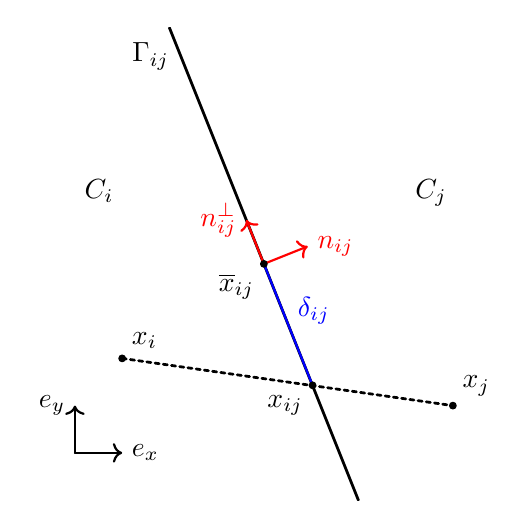
\begin{tikzpicture}[line cap=round,line join=round,x=1.0cm,y=1.0cm, scale = 0.6]
			\clip(-5,-5) rectangle (5.,5.);
			\draw [line width=1.pt] (-2,5.)-- (2,-5.);
			\draw[color=black] (-1.8,3.9) node[above left] {$\Gamma_{ij}$};
			\draw [line width=1.pt,dash pattern=on 1.5pt off 1.5pt] (-3,-2)-- (4,-3);
			\draw [color=red][->,line width=0.8pt] (0.,0.) -- (0.92847669,0.37139068);
			\draw[color=red] (0.92847669,0.37139068) node[right] {$n_{ij}$};
			\draw [color=red][->,line width=0.8pt] (0.,0.) -- (-0.37139068,0.92847669);
			\draw[color=red] (-0.37139068,0.92847669) node[left] {$n_{ij}^{\bot}$};
			\draw [color=blue][line width=0.8pt] (0.,0.) -- (1.03,-2.57);
			\draw[color=blue] (1.6,-1.) node[left] {$\delta_{ij}$};
			
			% Point
			\draw (-4,2) node[anchor=north west] {$C_i$};
			\draw (3,2) node[anchor=north west] {$C_j$};
			\draw[color=black] (-3,-2) node[above right] {$x_i$};
			\draw [fill=black] (-3,-2) circle (2.0pt);
			\draw[color=black] (4,-3) node[above right] {$x_j$};
			\draw [fill=black] (4,-3) circle (2.0pt);
			\draw[color=black] (0.,0.) node[below left] {$\overline{x}_{ij}$};
			\draw [fill=black] (0.,0.) circle (2.0pt);
			\draw[color=black] (1.03,-2.57) node[below left] {$x_{ij}$};
			\draw [fill=black] (1.03,-2.57) circle (2.0pt);
			%% \draw [fill=xdxdff] (8.778392298328422,5.318228205273862) circle (2.5pt);
			\draw[color=black] (8.863325183374085,5.53357142857143) node[right] {$\Gamma_{ij}$};
			%% Base cartésienne
			\draw [color=black][->,line width=0.8pt] (-4,-4) -- (-3,-4);
			\draw [color=black][->,line width=0.8pt] (-4,-4) -- (-4,-3);
			\draw[color=black] (-3,-4) node[ right] {$e_x$};
			\draw[color=black] (-4,-3) node[ left] {$e_y$};
		\end{tikzpicture}
		\captionof{figure}{Interface orientée $\Gamma_{ij}$ localisée entre deux cellules $C_i$ et $C_j$ d'un maillage non structuré $\mathcal{T}$ dont  le vecteur normal et son orthogonal sont représentés.}
		\label{fig:EdgeWithGrandeurs_VecNormal}
	\end{center}
	
	Il est important de remarquer que puisque $n_{i,j}$ est orthogonal à $\Gamma_{i,j}$, ainsi $\bar x_{i,j} - x_{i,j}$ est colinéaire à $n_{i,j}^\perp$. Ainsi il existe un unique réel $\delta_{i,j}$ qui vérifie $\bar x_{i,j}-x_{i,j} = \delta_{i,j}n_{i,j}^\perp$.\\
	Ainsi $M_i$ se reformule de la manière suivante :
	\begin{center}
		$M_i = I_2 - \dfrac1{\abs{C_i}}\displaystyle\sum_{j \in \mathcal N_i} \lambda_{i,j}\delta_{i,j} {n_{i,j}}\otimes n_{i,j}^\perp$
	\end{center}

	A partir de là il est possible d'obtenir une première propriété sur $M_i$ :
	
	\begin{lm}
		\begin{minipage}[t]{17cm}
			Soit $M_i(\mathcal T)$ la matrice $M_i$ associées au maillage $\mathcal T$.
		\end{minipage}
		
		\noindent\begin{minipage}{18cm}
			\hspace{.5cm}Soit $\mathcal T_1$ et $\mathcal T_2$ deux maillages el qu'il existe $\overline{C_{i_1}} \in \mathcal T_1$, $C_{i_2} \in \mathcal T_2$ et $h_\Omega$ une homothétie de rapport $k > 0$  tel que :
			\begin{enumerate}
				\item $h_\Omega(\overline{C_{i_1}}) = C_{i_2}$,
				\item $\overline{C_{i_1}}$ et $C_{i_2}$ possède le même nombre de voisins (ie. $\mathcal N_{i_1}(\mathcal T_1) = \mathcal N_{i_2 }(\mathcal T_2)$),
				\item $h_\Omega\big( \{ \text{voisins de $\overline{C_{i_1}}$} \} \big)= \{\text{voisins de $C_{i_2}$}\}$,
			\end{enumerate}
			alors : 
			\[ 
				M_{i_1}(\mathcal T_1) = M_{i_2}(\mathcal T_2)
			\]
		\end{minipage}
	\end{lm}
	\begin{dem}
		\begin{minipage}[t]{15cm}
			Soit $C_i \in \mathcal T$. Puisque toute homothétie conserve les angles et pour tout segment $I$
		\end{minipage}
		
		\noindent\begin{minipage}{18.5cm}
		 et surface $S$ :
		 \begin{enumerate}
		 	\item $\abs{h_\Omega(I)} = k\abs{I}$
		 	\item $\abs{h_\Omega(S)} = k^2\abs{S}$
		 \end{enumerate}
		 Soit $ \delta(C_i,C_i\cup C_j) = \delta_{i,j} $.\\
		 Puisque $k > 0$, $h_\Omega$ conserve aussi le sens des vecteurs, il suit la relation suivante : 
		 \[
		 	\delta(h_\Omega(C_i),h_\Omega(C_i) \cup h_\Omega(C_j)) =  \delta(h_\Omega(C_i),h_\Omega(C_i \cup C_j)) = k\delta_{i,j}
		 \]
		 Ainsi :
		\[
			\dfrac{\abs{h_\Omega(\Gamma_{i,j})}\delta(h_\Omega(C_i)\cup h_\Omega(C_j))}{\abs{h_\Omega(C_i)}} = \dfrac{k^2\lambda_{i,j}\delta_{i,j}}{k^2\abs{C_i}} = \dfrac{\lambda_{i,j}\delta_{i,j}}{\abs{C_i}}
		\]
		Puisque $h_{\Omega}$ conserve le sens et la direction, il vient $n_{i_1,j}(\mathcal T_1) = n_{i_2,j}(\mathcal T_2)$. Ainsi :
		\[
			\begin{aligned}
				M_{i_2}(\mathcal T_2) &= I_2 - \dfrac1{\abs{C_{i_2}}}\displaystyle\sum_{j \in \mathcal N_{i_2}(\mathcal T_2)} \lambda_{i_2,j}(\mathcal T_2)\delta_{i_2,j}(\mathcal T_2) n_{i_2,j}(\mathcal T_2)\otimes n_{i_2,j}(\mathcal T_2)^\perp\\
				&= I_2 - \dfrac1{\abs{h_\Omega(\overline{C_{i_1}})}}\displaystyle\sum_{j \in \mathcal N_{i_1}(\mathcal T_1)} \abs{h_\Omega(\Gamma_{i_1,j}(\mathcal T_1))}\delta(h_\Omega(\overline{C_{i_1}}),h_\Omega(\overline{C_{i_1}})\cup h_\Omega(\overline{C_j}))\; n_{i_1,j}(\mathcal T_1)\otimes n_{i_1,j}(\mathcal T_1)^\perp\\
				&=I_2 - \dfrac1{\abs{\overline{C_{i_1}}}}\displaystyle\sum_{j \in \mathcal N_{i_1}(\mathcal T_1)} \lambda_{i_1,j}(\mathcal T_1)\delta_{i_1,j}(\mathcal T_1) n_{i_1,j}(\mathcal T_1)\otimes n_{i_1,j}(\mathcal T_1)^\perp\\
				&= M_{i_1}(\mathcal T_1)
			\end{aligned}
		\]
		\end{minipage}
	\end{dem}
	
	Ce qui montre que ce qui influence la valeurs des coefficients de $M_i$ n'est pas les distances des cellules du maillage mais les angles dans chaque cellules et entre chaque cellules. Ce qui est d'autant plus clair à l'aide de la formule (29) donné par \cite{florent}, en notant $\theta_{i,j}$ l'unique angle tel que $n_{i,j} = \cos(\theta_{i,j}) e_x + \sin(\theta_{i,j})e_y$ et $\alpha_{i,j} = \frac{\lambda_{i,j}\delta_{i,j}}{\abs{C_i}}$ :
	\[
		\det(M_i) = 1 + \displaystyle\sum_{1\leq j < k \leq \mathcal N_i} \alpha_{i,j}\alpha_{i,k}\sin^2(\theta_{i,j}-\theta_{i,k})
	\]
	
	
	IL est possible d'obtenir des résultats plus fins dans le cas des maillage triangulaire. 
	
	\subsection{Majoration de $M_i^{-1}$}
	
	
	Soit $\mathcal M_2(\R)$ l'espace des matrice $2\times 2$ réels muni de la norme subordonnée à la norme $|\!|\cdot|\!|_2$, noté de la même manière.\\
	En examinant les valeurs propres de $M_i$, il est possible de déterminer $|\!|M_i^{-1}|\!|$.
	
	\begin{lm}\label{lm:maj_gen_Mi}
		Soit $\mathcal T$ un maillage, $i \in \mathcal T$ et $\alpha_i = \underset{j \in \mathcal N_i}\sum \alpha_{i,j}$.
		
		\begin{equation}
			|\!|M_i^{-1}|\!|_2 \leq \max_i \sqrt{\dfrac{4+\alpha_i^2 -2 \det(M_i) }{\det(M_i)^2}}.
		\end{equation}
	\end{lm}
	
	\subsection{Maillage Triangulaire}
	Pour pouvoir majorer $M_i^{-1}$ il a été vu qu'il suffisait de montrer que les $\alpha_{i,j}$ sont bornées et que les $\det(M_i)$ sont minorés par un réels strictement positif.	
	\par Pour obtenir un résultat plus précis, il faut pouvoir estimer précisément la valeur de $\alpha_{i,j} = \dfrac{\delta_{i,j}\lambda_{i,j}}{\abs{C_i}}$. Puisque $\lambda_{i,j}$ et $\abs{C_i}$ sont des données du maillages, il reste à déterminer$\delta_{i,j}$. Or $\abs{\delta_{i,j}} = |\!|x_{i,j}-\bar x_{i,j}|\!|$. Ce qui revient à étudier le système suivant.\\
	
	Soient $ABC_1$ et $ABC_2$ deux triangles non plats, $G_1$ et $G_2$ les centres de gravités de $ABC_1$ et $ABC_2$ respectivement, et $I$ le point d'intersection entre $[G_1G_2]$ et $[AB]$.
	
	\begin{center}
		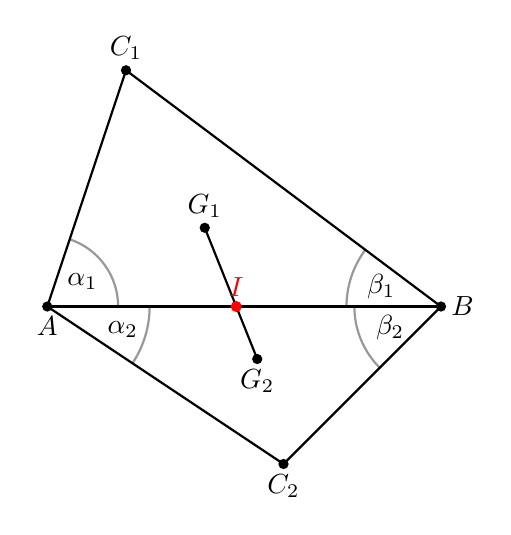
\begin{tikzpicture}[thick]
			\coordinate (A) at (0,0);
			\coordinate (B) at (5,0);
			\coordinate (C1) at (1,3);
			\coordinate (C2) at (3,-2);
			\coordinate (G1) at (barycentric cs:A=1,B=1,C1=1);
			\coordinate (G2) at (barycentric cs:A=1,B=1,C2=1);
			\draw (A)--(B)--(C1)--cycle;
			\draw (A)--(B)--(C2)--cycle;
			\draw[name path=ligne 1] (A)--(B);
			\draw[name path=ligne 2] (G1)--(G2);
			\fill[red,name intersections={of=ligne 1 and ligne 2,total=\t}]
			\foreach \s in {1,...,\t}{(intersection-\s) circle (2pt) node [above] {$I$}};
			
			\tkzMarkAngle[fill= orange,size=0.9cm,opacity=.4](B,A,C1)
			\tkzMarkAngle[fill= orange,size=1.3cm,opacity=.4](C2,A,B)
			\tkzLabelAngle[pos = 0.55](B,A,C1){$\alpha_1$}
			\tkzLabelAngle[pos = 1](C2,A,B){$\alpha_2$}
			
			\tkzMarkAngle[fill= orange,size=1.2cm,opacity=.4](C1,B,A)
			\tkzMarkAngle[fill= orange,size=1.1cm,opacity=.4](A,B,C2)
			\tkzLabelAngle[pos = 0.8](C1,B,A){$\beta_1$}
			\tkzLabelAngle[pos = 0.7](A,B,C2){$\beta_2$}
			
			\node [below] at (A) {$A$};
			\node [right] at (B) {$B$};
			\node [above] at (C1) {$C_1$};
			\node [below] at (C2) {$C_2$};
			\node [above] at (G1) {$G_1$};
			\node [below] at (G2) {$G_2$};
			
			\draw[fill=black] (A) circle (0.05cm);
			\draw[fill=black] (B) circle (0.05cm);
			\draw[fill=black] (C1) circle (0.05cm);
			\draw[fill=black] (C2) circle (0.05cm);
			\draw[fill=black] (G1) circle (0.05cm);
			\draw[fill=black] (G2) circle (0.05cm);
		\end{tikzpicture}
		\captionof{figure}{Deux triangles $ABC_1$ et $ABC_2$ de centre de gravité $G_1$ et $G_2$ respectivement. Et $\alpha_i,\beta_i \in ]0,\pi[$.}
	\end{center}
	
	Pour le lemme suivant, les notations suivantes sont adoptées : pour tout $n \in \N$ et $\mu_1,\mu_2 \in \R$, $\mu_n := \mu_{r+1}$, où $r$ est le reste de la division euclidienne de $n$ par 2.
	
	\begin{lm}
		En ce plaçant dans le contexte précédent, pour $k \in \{1,2\}$ :
		
		\noindent\begin{minipage}{15.5cm}
			\begin{equation}\label{eq:delta_angle_gauche}
			\frac{AB}2 - AI = \dfrac{AB-AC_k\cos(\alpha_k)}6 - \dfrac{AC_k\sin(\alpha_k)}3\dfrac{\cos(\alpha_{k+1})AC_{k+1} - \cos(\alpha_k)AC_k}{\sin(\alpha_k)AC_k+\sin(\alpha_{k+1})AC_{k+1}},
		\end{equation}
		et :
		\begin{equation}\label{eq:delta_angle_droit}
			\frac{AB}2 - BI = \dfrac{AB-BC_k\cos(\beta_k)}6 - \dfrac{BC_k\sin(\beta_k)}3\dfrac{\cos(\beta_{k+1})BC_{k+1} - \cos(\beta_k)BC_k}{\sin(\beta_k)BC_k+\sin(\beta_{k+1})BC_{k+1}}.
		\end{equation}
		\end{minipage}
	\end{lm}
	\begin{dem}
		\begin{minipage}[t]{18.5cm}
			Il sera d'abord traité le cas : $k=1$ pour l'équation (\ref{eq:delta_angle_gauche}), les autres suivants par symétrie.
		\end{minipage}
		\noindent\begin{minipage}{18.5cm}
			Il est possible de décrire les deux triangles à l'aide de coordonnées cartésienne. En effectuant une rotation et translation il est possible de supposer que $A=(0,0)$, $y_B = 0$ et $x_B >0$. Et à l'aide d'une symétrie axiale, il est possible de supposer sans restriction que $y_{C_1} > 0 > y_{C_2}$.\\
			
			Dans ce repère il possible d'écrire $G_1$ et $G_2$ en fonction de celle de $A,B,C_1$ et $C_2$ :\\ $G_k = \dfrac13\left(A+B+C_k\right) = \left(\frac{x_B+x_{C_k}}3,\frac{y_{C_k}}3\right)$. Pour déterminer les coordonnées de $I$, il suffit de paramétrer le segment $[G_1,G_2]$ de la manière suivante : $l(t) = (l_x(t),l_y(t)) = (1-t)G_1 + tG_2$ et de chercher $t_0$ de sorte que $l_y(t_0) = 0$.
			
			\[\begin{aligned}
					 && l_y(t_0) &=0,\\
				\iff && (1-t_0)y_{G_1} + t_0 y_{G_2} &= 0,\\
				\iff && t_0(y_{G_2}-y_{G_1})&=-y_{G_1},\\
				\iff && t_0(y_{C_2}-y_{C_1})&=-y_{C_1},\\
				\iff && t_0&=\dfrac{-y_{C_1}}{y_{C_2}-y_{C_1}}.
			\end{aligned}\]
			Ainsi, $x_I = l_x(t_0) = t_0(x_{G_2}-x_{G_1}) + x_{G_1} = -\dfrac{y_{C_1}}3\dfrac{x_{C_2}-x_{C_1}}{y_{C_2}-y_{C_1}} + \dfrac{x_B+x_{C_1}}3$. Et donc : 
			\[\frac{AB}2 - AI = \frac{x_B}2 - x_I = \dfrac{x_B-2x_{C_1}}6 + \dfrac{y_{C_1}}3\dfrac{x_{C_2}-x_{C_1}}{y_{C_2}-y_{C_1}}.\]
			En utilisant la formule du sinus et cosinus, il vient : 
			\[\begin{aligned}
				\frac{AB}2 - AI &= \dfrac{AB-2AC_1\cos(\alpha_1)}6 + \dfrac{AC_1\sin(\alpha_1)}3\dfrac{AC_2\cos(\alpha_2)-AC_1\cos(\alpha_1)}{-AC_2\sin(\alpha_2)-AC_1\sin(\alpha_1)}\\
			& = \dfrac{AB-2AC_1\cos(\alpha_1)}6 - \dfrac{AC_1\sin(\alpha_1)}3\dfrac{AC_2\cos(\alpha_2)-AC_1\cos(\alpha_1)}{AC_2\sin(\alpha_2)+AC_1\sin(\alpha_1)}
			\end{aligned}\]
			
			Par symétrie il vient les 3 autres équations.
		\end{minipage}
	\end{dem}
	
	En testant différentes configurations sur un logiciel de géométrie dynamique il vient assez naturellement de constater qu'une condition intéressante est la convexité du quadrilatère $AC_1BC_2$, il vient alors $\abs{AB/2-AI} \leq \frac{AB}6$. C'est ce qui est démontré ci-dessous.
	
	\begin{lm}\label{lm:maj_delta_triangle}
		Si le quadrilatère $AC_1BC_2$ est convexe alors :
		\begin{equation}
			\abs{\frac{AB}2-AI} \leq \frac{AB}6
		\end{equation}
	\end{lm} 
	\begin{dem}
		\begin{minipage}[t]{16.5cm}
			Dans cette preuve, il sera traité le cas où $AB/2 \geq AI$, l'autre cas se traitant strictement de la même manière en considérant : $BI = AB-AI$ à la place de $AI$.
		\end{minipage}
		
		\noindent\begin{minipage}{18.5cm}
			Puisque $AC_1BC_2$ est convexe, il vient que $\alpha_1+\alpha_2 \leq \pi$ (sinon $[C_1C_2]$ n'est pas dans $AC_1BC_2$). Soit $k \in\{1,2\}$.\\
			
			Ainsi : $\abs{\frac{AB}2-AI} = \dfrac{AB-2AC_k\cos(\alpha_k)}6 - \dfrac{AC_k\sin(\alpha_k)}3\dfrac{AC_{k+1}\cos(\alpha_{k+1})-AC_k\cos(\alpha_k)}{AC_{k+1}\sin(\alpha_{k+1})+AC_k\sin(\alpha_k)}$.\\
			
			Ainsi pour trouver un majorant $\abs{AB/2-AI}$ il convient de minimiser $\dfrac{AC_{k+1}\cos(\alpha_{k+1})-AC_k\cos(\alpha_k)}{AC_{k+1}\sin(\alpha_{k+1})+AC_k\sin(\alpha_k)}$ en la variable $\alpha_{k+1}$ car $\sin(\alpha_k)\geq 0$.\\
			Il faut donc étudier la fonction suivante : $f(x) = \dfrac{AC_{k+1}\cos(x)-AC_k\cos(\alpha_{k+1})}{AC_{k+1}\sin(x)+AC_k\sin(\alpha_k)}$ qui est continue et dérivable :
			\[
				\begin{aligned}
					&\left(AC_{k+1}\sin(x)+AC_k\sin(\alpha_k)\right)^2f'(x) \\
					=& -AC_2\sin(x)\left(AC_{k+1}\sin(x)+AC_k\sin(\alpha_k)\right) - AC_{k+1}\cos(x)\left(AC_{k+1}\cos(x)-AC_k\cos(\alpha_k)\right)\\
					=&-AC_{k+1}^2\left(\cos(x)^2+\sin(x)^2\right) + AC_kAC_{k+1}\left(\cos(\alpha_k)\cos(\alpha_{k+1})-\sin(\alpha_k)\sin(\alpha_{k+1})\right)\\
					=&-AC_{k+1}^2 + AC_kAC_{k+1}\cos(\alpha_k+\alpha_{k+1})\\
					=&AC_{k+1}(AC_k\cos(\alpha_k+\alpha_{k+1})-AC_{k+1})
				\end{aligned}
			\]
			Si $\alpha_1+\alpha_2 \geq \pi/2$, alors $\cos(\alpha_1+\alpha_2) \leq 0$. Et si $\alpha_1+\alpha_2 \leq \pi/2$, il est possible de choisir $k$ de sorte que $AC_k\cos(\alpha_k+\alpha_{k+1})-AC_{k+1} \leq 0$, car si $AC_1\cos(\alpha_1+\alpha_2)-AC_2 > 0$ et $AC_2\cos(\alpha_1+\alpha_2)-AC_1 > 0$, alors $AC_1\cos(\alpha_1+\alpha_2)^2 \geq AC_2\cos(\alpha_1+\alpha_2) > AC_1$, ce qui implique : $AC_1\cos(\alpha_1+\alpha_2) > AC_1$, ce qui est absurde. Il est ainsi possible de choisir un tel $k \in \{1,2\}$. Ainsi :
			\[
			\begin{aligned}
				\abs{\frac{AB}2 - AI} &\leq \dfrac{AB-2AC_1\cos(\alpha_1)}6 - \dfrac{AC_1\sin(\alpha_1)}3f(\pi-\alpha_1),\\
				&\leq \dfrac{AB-2AC_1\cos(\alpha_1)}6 + \dfrac{AC_1\sin(\alpha_1)}3\dfrac{AC_2\cos(\alpha_1)+AC_1\cos(\alpha_1)}{AC_2\sin(\alpha_1)+AC_1\sin(\alpha_1)},\\
				&\leq \dfrac{AB-2AC_1\cos(\alpha_1)}6 + \dfrac{AC_1\cos(\alpha_1)}3,\\
				&\leq \dfrac{AB}6.
			\end{aligned}
			\]
		\end{minipage}
	\end{dem}
	
	
	
	De ce lemme, il est immédiatement possible de déduire la majoration suivante :
	
	\begin{lm}
		\begin{minipage}[t]{15cm}
			Soit $\mathcal T$ une triangulation telle que l'union tout couple de triangles voisins est convexe, alors pour tout $i \in \mathcal T$ et $j \in \mathcal N_i$ :
		\end{minipage}
		\begin{equation}\label{eq:maj_delta}
			|\!|x_{i,j} - \bar x_{i,j}|\!| \leq \frac{\lambda_{i,j}}6
		\end{equation}
	\end{lm}
	\begin{dem}
		\begin{minipage}[t]{15cm}
			Soit $T_i \in \mathcal T$ et $j \in \mathcal N_i$. Soit $A$ et $B$ les sommets de $\Gamma_{i,j}$, $C_1$ le sommet opposé à $\Gamma_{i,j}$ de $T_i$, $C_2$ le sommet opposé à $\Gamma_{i,j}$ de $T_j$.
		\end{minipage} 
		
		\noindent\begin{minipage}{16cm}
			Il vient alors : $|\!|x_{i,j} -\bar x_{i,j}|\!| = |\!| x_{i,j}-A - (\bar x_{i,j}-A)|\!| = \abs{Ax_{i,j}-A\bar x_{i,j}}$. Or $A\bar x_{i,j} = AB/2$. Donc $|\!|x_{i,j} -\bar x_{i,j}|\!| = \abs{AB/2-A\bar x_{i,j}}$. Ainsi d'après le lemme \ref{lm:maj_delta_triangle} : $\abs{AB/2-A\bar x_{i,j}}\leq \frac{AB}6 = \frac{\lambda_{i,j}}6 $ .\\
			Finalement, $|\!|x_{i,j} -\bar x_{i,j}|\!| \leq \frac{\lambda_{i,j}}6$.
		\end{minipage}
	\end{dem}
	
	Il est maintenant possible de majorer $\alpha_{i,j}$ à l'aide de la notation suivante :
	
	\begin{center}
		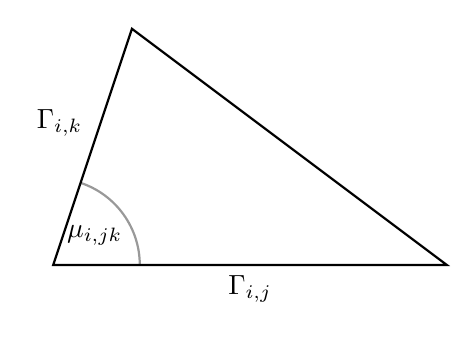
\begin{tikzpicture}[thick]
			\coordinate (A) at (0,0);
			\coordinate (B) at (5,0);
			\coordinate (C1) at (1,3);
			\coordinate (M1) at (barycentric cs:A=1,B=1);
			\coordinate (M2) at (barycentric cs:A=1,C1=1);
			\draw (A)--(B)--(C1)--cycle;
			\draw (M1) node [below] {$\Gamma_{i,j}$};
			\draw (M2) node [above left] {$\Gamma_{i,k}$};
			
			\tkzMarkAngle[fill= orange,size=1.1cm,opacity=.4](B,A,C1)
			\tkzLabelAngle[pos = 0.65](B,A,C1){$\mu_{i,jk}$}

		\end{tikzpicture}
		\captionof{figure}{Illustration d'une cellule $C_i$, avec $\mu_{i,jk} \in ]0,\pi[$ l'angle formé par $\Gamma_{i,j}$ et $\Gamma_{i,k}$.}
	\end{center}
	
	\begin{lm}\label{lm:majoration_alpha}
		\begin{minipage}[t]{18.5cm}
			Soit $\mathcal T$ une triangulation telle que l'union de tout couple de triangles voisins est convexe.
		\end{minipage}
		Pour tout $k,j \in \mathcal N_i$ tel que $k \not = j$,
		\begin{equation}
			\abs{\alpha_{i,j}} \leq \dfrac{\lambda_{i,j}}{3\lambda_{i,k}\sin(\mu_{i,jk})}
		\end{equation}
	\end{lm}
	
	Et il vient immédiatement :

	\begin{lm}\label{lm:majoration_produit_alpha}
		\begin{minipage}[t]{18.5cm}
			Soit $\mathcal T$ une triangulation telle que l'union de tout couple de triangles voisins est convexe.
		\end{minipage}
		Pour tout $k,j \in \mathcal N_i$ tel que $k \not = j$,
		\begin{equation}
			\abs{\alpha_{i,j}\alpha_{i,k}} \leq \dfrac{1}{9\sin^2(\mu_{i,jk})}
		\end{equation}
	\end{lm}
	
	Avant passer à la minoration du déterminant, il est nécessaire de faire le lien entre $\sin^2(\mu_{j,k})$ et $\sin^2(\theta_{i,j}-\theta_{i,k})$.
	
	\begin{lm}
		\begin{minipage}[t]{18.5cm}
			Soit $\mathcal T$ une triangulation. Alors pour tout $j \not = k \in \mathcal T$ :
		\end{minipage}
		\begin{equation}
			\sin^2(\mu_{i,jk}) = \sin^2(\theta_{i,j}-\theta_{i,k})
		\end{equation}
	\end{lm}
	
	Il est maintenant possible de minorer le déterminant de $M_i$.
	
	\begin{lm}\label{lm:maj_det}
		\begin{minipage}[t]{18.5cm}
			Soit $\mathcal T$ une triangulation telle que l'union de tout couple de triangles voisins est convexe.
		\end{minipage}
		Alors pour tout $i \in\mathcal{T}$ et $j \in \mathcal N_i$ :
		\begin{equation}
			\det(M_i) \geq \dfrac23
		\end{equation}
	\end{lm}
	
	Pour pouvoir donner une majoration intéressante de $M_i^{-1}$, il reste à savoir s'il est possible de majorer les $\abs{\alpha_{i,j}}$, ce qui va dépendre fortement de l'angle minimum atteint.
	
	\begin{lm}
		Soit $\mathcal T$ une triangulation.
		
		
		\begin{minipage}{15.5cm}
			S'il existe $\mu_{\min} > 0$ tel que pour tout $i \in \mathcal T$ et $j \not = k \in \mathcal T$, $\mu_{i,jk} \geq \mu_{\min}$ :
			
			\[
				\abs{\alpha_{i,j}} \leq \dfrac1{\sin(\mu_{\min})}
			\]
		\end{minipage}
	\end{lm}
	
	Il est maintenant possible de fournir une majoration intéressante de $M_i{-1}$ sous certaines conditions qui sont détaillés ci-dessous :
	
	\begin{lm}
		Soit $\mathcal T$ un maillage triangulaire.\\
		\begin{minipage}[t]{18.5cm}
			Si l'union de tout couple de triangles voisins est convexe et il existe $\mu_{\min} > 0$ pour tout $i \in \mathcal T$, $j \not = k \in \mathcal N_i$, $\mu_{i,jk} \geq \mu_{\min}$. Alors pour tout $i \in \mathcal T$,
		\end{minipage}
		\begin{equation}
			|\!|M_i^{-1}|\!|_2 \leq \sqrt{30+\frac{81}{\sin^2(\mu_{\min})}}.
		\end{equation}
	\end{lm}
	
\section{Tests numériques}

\subsection{Objectifs}

L'objectif est ici de confirmer sur différents maillages les ordres de convergences trouvé pour le pas $h_2$ dont la formule est donné en (\ref{eq:nv_h}). L'objectif est ici de mesurer l'erreur $E_k(h_2) = \max_{i\in\mathcal T} |\!| \overline{\nabla u(x_i)} - \nabla u_i |\!|_k $ où $k = 1$ ce qui permet de moyenné l'erreur et de retrouver l'ordre plus facilement, $k = 2$ pour la moyenne quadratique et est plus sensible encore, et, pour $k=\infty$ pour l'erreur en norme infinie qui donne une mesure de l'erreur encore plus fine et ainsi beaucoup plus sensible. L'objectif est de retrouver : $E_k(h_2) = \mathcal O(h_2)$.\\

La fonction $u$ choisie pour estimer l'erreur est bien connue et très régulière : 
\[u(x,y) = \exp\left(\dfrac{(x-x_c)^2+(y-y_c)^2}{2\sigma^2}\right),\]
c'est une gaussienne centré en $(x_c,y_c)$ et de variance $\sigma^2$. Elle est donc clairement d'ordre $\mathcal C^2$.\\
De plus, le gradient de cette fonction est très bien connu :
\[
\nabla u(x,y) = u(x,y)\begin{bmatrix}
	-\frac{x-x_c}{\sigma^2}\\
	-\frac{y-x_c}{\sigma^2}
\end{bmatrix}
\]
Ainsi les $u_i$ et $\nabla u_i$ sont connus avec exactitude et permet ainsi de mesurer l'erreur avec exactitude.

\subsection{Matériels}

Pour tester ce gradient discret, il a été choisi de prendre un domaine $\Omega$ à mailler de forme carré : $ \Omega = [0,\;10]\times[0,\;10]$ sur lequel a été appliqué différents maillages dans cet ordre :
\begin{enumerate}
	\item Maillage cartésien (des rectangles de taille $\frac N{10}$ par $\frac M{10}$).
	\item Maillage avec une triangulation de type Delaunay généré à l'aide du mailleur FreeFem++.
	\item Maillage cartésien déformé qui se construit de la manière suivante :
	\begin{enumerate}
		\item construction d'un maillage cartésien comme en 1,
		\item Déformation des points à l'aide d'une variable aléatoire $r$ uniformément distribué sur $[-1,\;1]$, de $\Delta x = \frac N{10}$, de $\Delta y = \frac M{10}$ et d'un facteur de déformation $\varphi \in [0,\; 1]$ : 
		\[
			P^{perturbe}_{i,j} = P_{i,j} + \varphi r \left(\frac{\Delta x}2,\; \frac{\Delta y}2 \right)^t
		\]
	\end{enumerate}
\end{enumerate}

Le domaine $\Omega$ n'étant pas ouvert, et de plus à terme l'objectif est de résoudre des problème sur le plan en entier, il a été choisi de mettre des conditions de bord périodique. De plus la fonction test choisi étant une gaussienne centré au centre du maillage, $(x_c,y_c) = (5,5)$, la fonction prends au bord du domaine des valeurs très proche de 0, rendant nul les erreurs au bords du domaine, permettant ainsi de ne pas prendre en compte les conditions de bords.

\subsection{Maillage cartésien}

Pour obtenir l'ordre de convergence, il est généré plusieurs maillages en faisant varier le nombre de cellules. Voici un exemple d'un tel maillage pour $N=10$ points sur chaque côtés :

\begin{figure}[h]
	\centering
	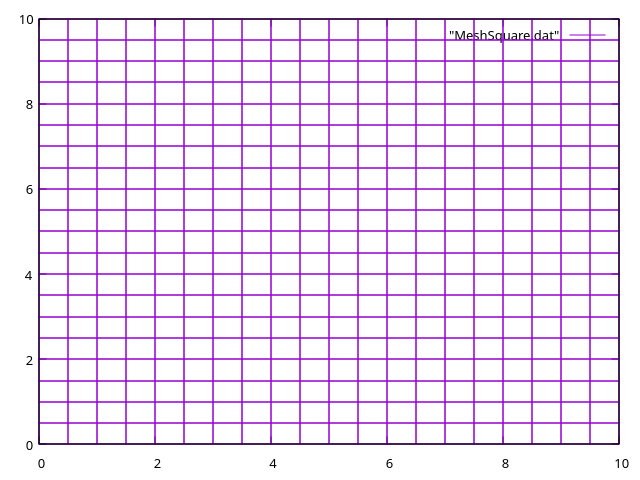
\includegraphics[scale=.3]{image/maillage_carre.png}
	\caption{Exemple de maillage cartésien pour 20 points par arrêtes}
\end{figure}

Voici les erreurs en fonction du pas :

\begin{figure}[h]
	\centering
	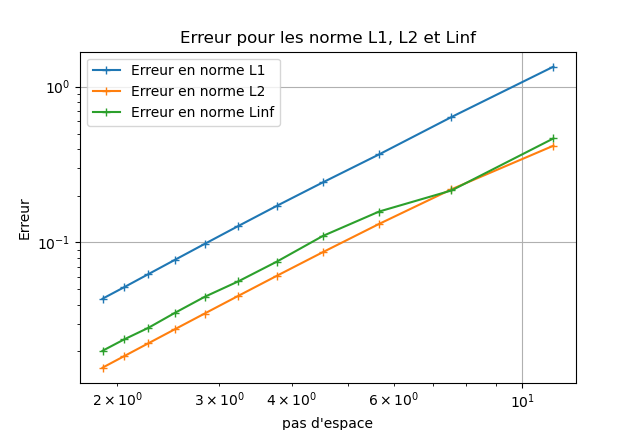
\includegraphics[scale=.7]{image/carre.png}
	\caption{Graphique des erreur en échelle logarithmique pour des maillages cartésiens}
\end{figure}

L'ordre 2 est bien retrouvé en faisant une régression linéaire sur le logarithme de l'erreur :
\begin{enumerate}
	\item[$\star$] Pour la norme $\mathrm L^1$, l'ordre de convergence $\simeq 1,917$
	\item[$\star$] Pour la norme $\mathrm L^2$, l'ordre de convergence $\simeq 1,855$
	\item[$\star$] Pour la norme $\mathrm L^\infty$, l'ordre de convergence $\simeq 1,744$
\end{enumerate}


\subsection{Maillage cartésien déformé}

Ici, pour obtenir l'ordre de convergence, il est fait de même que pour le cas des maillages cartésiens : le nombre de cellules est augmenté. Il faut aussi choisir un coefficient de déformation $\varphi \in [0,1]$. Voici un exemple de maillage pour 10 points sur chaque arrêtes et un coefficient de déformation de 0.9 :\\\\

\begin{figure}[h]
	\centering
	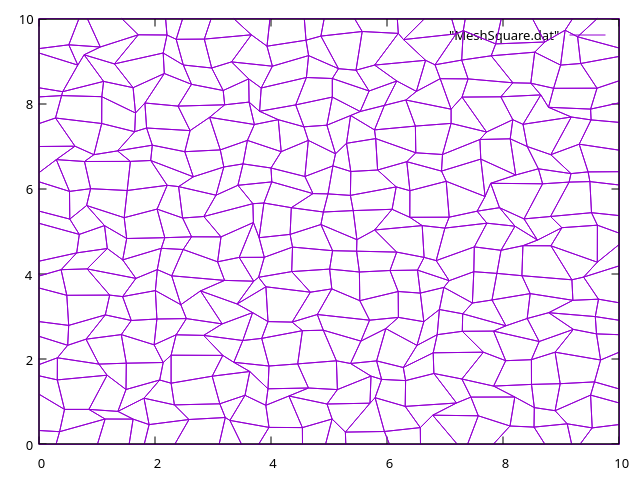
\includegraphics[scale=0.5]{image/maillage_deforme_09.png}
	\caption{Exemple de maillage cartésien déformé, de déformation $\varphi = 0.9$}
\end{figure}

Pour rappel, le maillage cartésien correspond exactement au coefficient de déformation $\varphi = 0$.

\subsubsection{Coefficient de déformation $\varphi = 0.2$}

\begin{figure}[h]
	\centering
	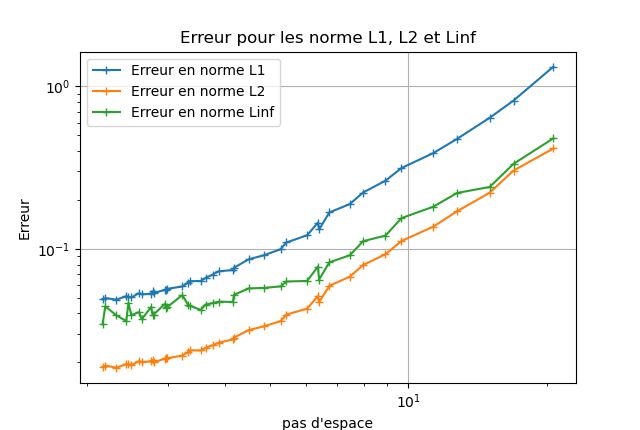
\includegraphics[scale=0.7]{image/deforme_02.png}
	\caption{Graphique des erreur en échelle logarithmique pour un maillage cartésien déformé, de déformation $\varphi = 0.2$.}
\end{figure}

On retrouve bien l'ordre de convergence de \textbf{1} pour les normes $\mathrm L^1$, $\mathrm L^2$ et $\mathrm L^\infty$ :
\begin{enumerate}
	\item[$\star$] Pour la norme $\mathrm L^1$, l'ordre de convergence $\simeq 1,413$
	\item[$\star$] Pour la norme $\mathrm L^2$, l'ordre de convergence $\simeq 1,357$
	\item[$\star$] Pour la norme $\mathrm L^\infty$, l'ordre de convergence $\simeq 1,034$
\end{enumerate}


\subsubsection{Coefficient de déformation $\varphi = 0.5$}

\begin{figure}[h]
	\centering
	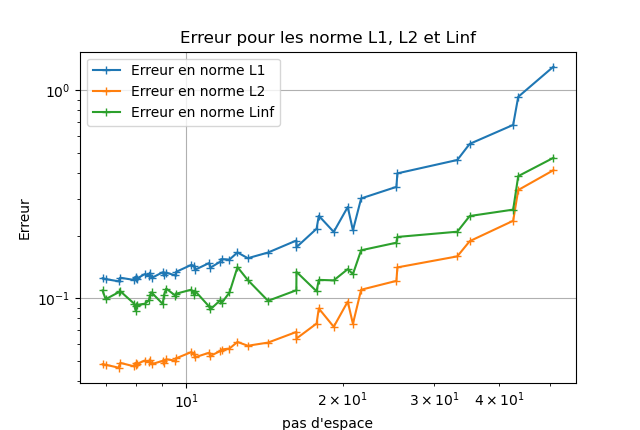
\includegraphics[scale=0.7]{image/deforme_05.png}
	\caption{Graphique des erreur en échelle logarithmique pour un maillage cartésien déformé, de déformation $\varphi = 0.5$.}
\end{figure}

On retrouve bien l'ordre de convergence de \textbf{1} pour les normes $\mathrm L^1$ et $\mathrm L^2$. Mais un peu dégradé pour $\mathrm L^\infty$ :
\begin{enumerate}
	\item[$\star$] Pour la norme $\mathrm L^1$, l'ordre de convergence $\simeq 1,029$
	\item[$\star$] Pour la norme $\mathrm L^2$, l'ordre de convergence $\simeq 0,951$
	\item[$\star$] Pour la norme $\mathrm L^\infty$, l'ordre de convergence $\simeq 0,632$
\end{enumerate}

\subsubsection{Coefficient de déformation $\varphi = 0.8$}

\begin{figure}[h]
	\centering
	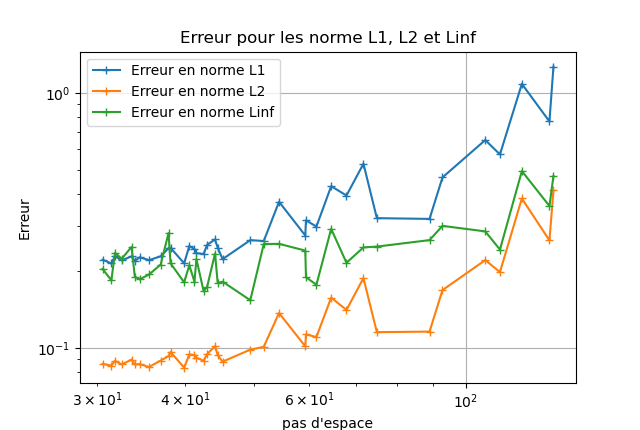
\includegraphics[scale=0.7]{image/deforme_08.png}
	\caption{Graphique des erreur en échelle logarithmique pour un maillage cartésien déformé, de déformation $\varphi = 0.2$.}
\end{figure}

On retrouve bien l'ordre de convergence de \textbf{1} pour les normes $\mathrm L^1$ et $\mathrm L^2$. Mais pour la norme $\mathrm L^\infty$:
\begin{enumerate}
	\item[$\star$] Pour la norme $\mathrm L^1$, l'ordre de convergence $\simeq 0.964$
	\item[$\star$] Pour la norme $\mathrm L^2$, l'ordre de convergence $\simeq 0,862$
	\item[$\star$] Pour la norme $\mathrm L^\infty$, l'ordre de convergence $\simeq 0,416$
\end{enumerate}




\subsubsection{Coefficient de déformation $\varphi = 0.9$}

\begin{figure}[h]
	\centering
	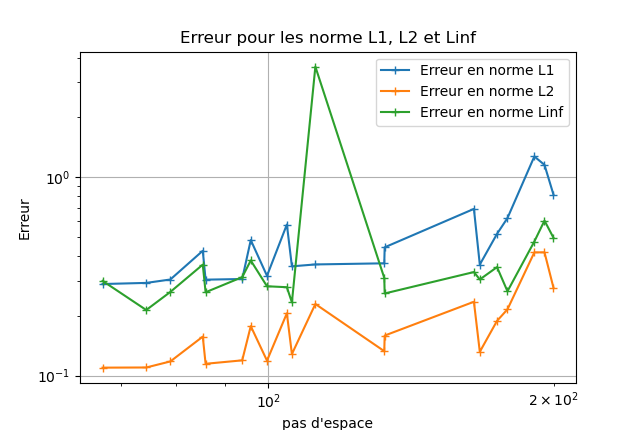
\includegraphics[scale=0.7]{image/deforme_09.png}
	\caption{Graphique des erreur en échelle logarithmique pour un maillage cartésien déformé, de déformation $\varphi = 0.2$.}
\end{figure}

On retrouve bien l'ordre de convergence de \textbf{1} pour les normes $\mathrm L^1$ et $\mathrm L^2$. Mais pas pour la norme $\mathrm L^\infty$ :
\begin{enumerate}
	\item[$\star$] Pour la norme $\mathrm L^1$, l'ordre de convergence $\simeq 1,001$
	\item[$\star$] Pour la norme $\mathrm L^2$, l'ordre de convergence $\simeq 0,891$
	\item[$\star$] Pour la norme $\mathrm L^\infty$, l'ordre de convergence $\simeq 0,364$
\end{enumerate}



\subsubsection{Observations}

Il peut être constaté que l'ordre de convergence se dégrade au fur et à mesure que l'on augmente le coefficient de déformation, seulement une soudaine dégradation de l'ordre de convergence est constaté lors du passage de $\varphi=0.8$ à $\varphi=0.9$, notamment pour la norme $\mathrm L^\infty$.
\par De plus, il est constaté que plus le coefficient de déformation augmente plus il est difficile de raffiner le pas $h_2$, en effet, le pas minimum (pour un même échantillon de maillage, dans le sens où pour chaque déformation on a testé pour un ensemble de maillage dont le nombre de maille est le même) est de plus en plus grand.



\subsection{Maillage de Delaunay}

Ici, pour obtenir l'ordre de convergence, il est fait de même que pour le cas des maillages cartésiens : le nombre de cellules est augmenté. Voici un exemple de maillage pour peu de cellules :

\begin{figure}[h]
	\centering
	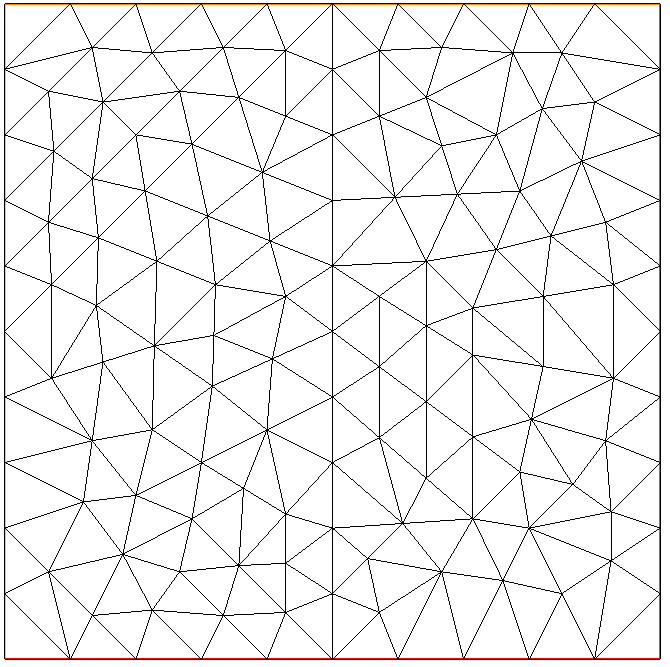
\includegraphics[scale=0.5]{image/maillage_ffm.png}
	\caption{Exemple de maillage de Delaunay pour 10 points sur chaque arrêtes}
\end{figure}

\newpage

Voici les courbes de convergences associés aux normes respectives :

\begin{figure}[h]
	\centering
	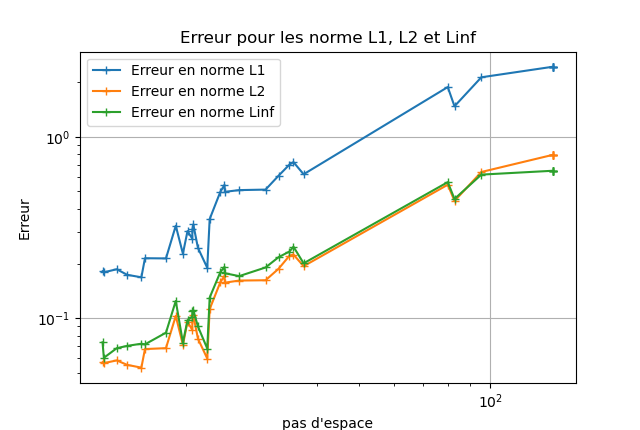
\includegraphics[scale=0.7]{image/ffm.png}
	\caption{Graphique des erreur en échelle logarithmique pour des maillages de Delaunay.}
\end{figure}


On retrouve bien l'ordre de convergence de \textbf{1} pour les normes $\mathrm L^1$, $\mathrm L^2$ et $\mathrm L^\infty$ :
\begin{enumerate}
	\item[$\star$] Pour la norme $\mathrm L^1$, l'ordre de convergence $\simeq 1,144$
	\item[$\star$] Pour la norme $\mathrm L^2$, l'ordre de convergence $\simeq 1,149$
	\item[$\star$] Pour la norme $\mathrm L^\infty$, l'ordre de convergence $\simeq 0,996$
\end{enumerate}




\newpage

\begin{thebibliography}{99}	
	\bibitem{ludo}
	L. Martaud,
	Global entropy stability for a class of unlimited second-order schemes for 2D hyper-bolic systems of conservation laws on unstructured meshes.
	 Journal of Computational Physics,
	487 :112176, 2023.
	
	\bibitem{florent}
	P. Florent,
	Étude de l'anisotropie locale de maillages non-structurés 2D.
\end{thebibliography}
\end{document}